\documentclass[preprint2]{aastex}

\usepackage{url}
\usepackage{multirow}
\usepackage{amsmath}
\usepackage{xcolor}
\usepackage{mathrsfs}
%\citestyle{aa}



\newcommand{\etal}{{et al.\/}}
\newcommand{\Prob}{\mathtt{P}}
\newcommand{\logL}{\log\mathcal{L}}
\newcommand{\unit}[1]{\footnotesize #1}
\newcommand{\PAPER}{\mathrm{PAPER}}
\newcommand{\hMpci}{h\ {\rm Mpc}^{-1}}

\newcommand{\Nx}{$N_x$}
\newcommand{\MminX}{$M_{minX}$}
\newcommand{\alphaX}{$\alpha_X$}
\newcommand{\xray}{X-ray}

\newcommand{\HI}{HI}
%%define graphics path to search for images
%\graphicspath{{./data/}}

%\usepackage[justification=centering]{caption}

\definecolor{orange}{RGB}{255,127,0}

\tabletypesize{\scriptsize}

	% End definitions

%\slugcomment{DRAFT: \today}

\shorttitle{ECHO}
\shortauthors{Jacobs et al.}

\begin{document}


\title{The External Calibrator for Hydrogen Arrays}
\author{
Daniel C. Jacobs\altaffilmark{1},
Jacob Burba\altaffilmark{1},
Judd Bowman\altaffilmark{1},
Lauren Turner\altaffilmark{1},
Kali Johnson\altaffilmark{1}}
\altaffiltext{1}{School of Earth and Space Exploration, Arizona State U., Tempe, AZ, 85287}

\setcounter{footnote}{1}


\begin{abstract}
We describe the External Calibrator for Hydrogen Observatories (ECHO)
\end{abstract}



\section{Introduction}\label{sec:intro}

A new generation of radio arrays is being developed that use large numbers of low-cost elements, such as phased tiles of dipole antennas. This is made possible by developments in digital technology and enables exploration of new windows on the universe such as the epoch of reionization (EoR) via the redshifted 21 cm line (Morales \& Wyithe 2010; Madau et al. 1997; Loeb \& Zaldarriaga 2004; Loeb \& Barkana 2001; Furlanetto et al. 2006). Precise calibration of the primary beams of these dipole arrays has been found to be crucial to analysis of observations from the the Murchison Widefield Array (MWA; Tingay et al. (2013); Bowman et al. (2013)), the Precision Array for Probing the Epoch of Reionization (PAPER; Pober et al. (2013); Parsons et al. (2010); Jacobs et al. (2011)), and the Low Frequency Array (LOFAR; Yatawatta et al. (2013)). Beam calibration of low frequency dipole arrays poses several complications compared to traditional dish antennas. Most notable is that holographic beam calibration is not possible because the dipole array beams are steered electronically and are unique at every pointing direction. Drift scan calibration of dipole array beams is possible, but requires the test antenna/array to be embedded within an existing array that generates sufficient sensitivity to isolate a large number of radio sources to provide many tracks through the beam. Pober et al. (2012) have employed symmetry arguments to reduce the needed number of sources on the sky and improve the result for PAPER antennas, but this is not possible in general for more complicated dipole array beam patterns. Attempts have been made to use anechoic chambers to calibrate low-frequency phased arrays, but the measurements suffer since even the largest chambers cannot extend into the farfield pattern and the RF absorber material used in the chambers performs poorly below 150 MHz, creating reflections and resonances. Mapping of the dipole beams using the Orbcomm constellation of satellites has proven effective (Neben, Bradley and Hewitt in prep) but is limited to only a single frequency (138 MHz).



%The work proposed here will develop a method for directly measuring, in-situ, the response of dipoles, phased array tiles, and other experimental low-frequency receptors, particularly new elements proposed for the second generation Hydrogen Epoch of Reionization Array (HERA). The proposed method use a remotely controlled unmanned aerial vehicle equipped with a calibrated transmitting antenna and GPS and inertial position loggers to provide a known mulit-frequency reference signal for calibrating low-frequency antennas. Substantial initial development work has been performed already to design and characterize a prototype system. Here, we request modest funds (\$99,187 over two years) to support the implementation of a mature, deployable system based on our prototype efforts. A team of undergraduates, led by one postdoc (0.1 FTE), will assemble and field the prototype in a series of field experiments with the goal of routinely mapping the primary beams of several low frequency arrays, including the HERA prototype antenna installation outside Berkeley, CA.



\section{Design and Method}



\begin{comment}
The ECHO system utilizes two networked machines which will henceforth be referred to as the ground station (GS) and the accumulation station (AS).  Each station handles a different data stream, being GPS data for the GS and radio spectrum data for the AS.  % mention realtime accumulation?

For the calibration source, ECHO employs a X8 octoquad drone manufactured by 3DRobotics (3DR) with an onboard, programmable Valon 5007 synthesizer and a BicoLOG 30100 biconical antenna (see Fig.~\ref{fig:drone}).  To cover a large portion of the sky of the antenna under test (AUT), a spiral path along the surface of a sphere centered on the AUT with a radius greater than or equal to the AUT's far field distance is used.  The waypoints are generated using a Healpix map, which divides the sky up into pixels with equal area according to a user specified parameter $N_{side}$, a power of 2, and a total pixel count of $N_{pix}=12\times N_{side}^2$.  Ordered by pixel number from zenith to nadir, the altitude and azimuth of each pixel is obtained and converted to a waypoint, i.e. a list of waypoint number, latitude, longitude, and altitude.  These obtained waypoints are then written to a waypoint file in order of position, starting at the horizon and ending at zenith.  The internal GPS of the drone can then read in the generated waypoint file and autonomously follow these waypoints in flight.  A region of interest (ROI) can be declared in the waypoint file prior to the first waypoint to force the drone to always face a specific region and keep a fixed yaw, i.e. a fixed BicoLOG polarization

\cite{2005ApJ...622..759G}

To obtain the GPS position of the drone, MAVProxy\footnote{https://github.com/Dronecode/MAVProxy}, a ground control station written in Python implementing the MAVLink communication protocol, is used to facilitate communication between the drone and APM Planner\footnote{http://planner.ardupilot.com/planner2/index.html} on the GS. Through a TCP connection with APM Planner (the server) and the drone (the client), APM Planner records the latitude, longitude, and altitude of the drone with an associated timestamp at which the position was measured every ~300 ms.  These positions, along with many other intermittent parameters and error messages, are continuously written to a telemetry log (tlog) file.  This tlog is read and the realtime positions of the drone are recorded to a text file and made available for the AS via a queryable server setup on the GS.

In flight, the Valon synth is set to broadcast at a set frequency and power in the range of 137.5-4400 MHz.  A Signal Hound (SH) BB60A 9 kHz to 6 GHz spectrum analyzer is used to measure the signal received by the AUT which records a radio spectrum in dB with an associated timestamp.  The bandwidth of the recorded spectrum and its associated resolution can be modified based upon user input parameters pertaining to the number of FFT bins, the central frequency, and the bandwidth which cannot exceed 20 MHz.  The radio spectrum data is then read in and each time associated with a spectrum is used to query the server on the GS.  The output of which is an interpolated GPS position in the form of latitude, longitude, and altitude.  If there is no valid GPS data at the query time, then -1 is returned for each of the aforementioned values.  An accumulated file containing each query time and the associated latitude, longitude, altitude, and radio spectrum is then generated and used to produce a FITS file containing the primary beam response of the AUT.

\end{comment}


\section{Calibration}

The first full scale test of the ECHO system was done in August, 2015 at the National Radio Astronomy Observatory (NRAO) site in Green Bank, WV.  Two dual-polarization dipoles (see Fig.~\ref{fig:dual dipole}) used in the development of a calibration technique utilizing the ORBCOMM satellite constellation (Neben et al. 2015) were used as the AUTs.  With a dipole length of 90.4 cm and a Valon synth frequency of 137.554 MHz\footnote{Is this the right frequency}, a flight radius of 100m was chosen, well into the far-field of the dipoles.  Choosing a flight speed of 0.2 dam s$^{-1}$ and $N_{side}=8$, each flight ECHO performed took ~60 min.  Four total flights were performed as each antenna contained two dipoles and thus needed to be tested with two flights, one with a polarization of the BicoLOG matching the polarization of one of the dipoles.  This also allowed cross-polarization measurements of each antenna to be made.


\subsection{Maps}

The resulting maps can be seen somewhere... eventually...

\subsection{Comparison to Orbcomm Ratio Maps}
\section{MWA Tile}
\subsection{Data}
\subsection{Systematic Variation}
\subsection{Comparison to Orbcomm Maps}
\section{Conclusion}


\section{Acknowledgments}{

ECHO is supported by a grant from the National Science Foundation (NSF; award number 1407646). D.C.J would like to acknowledge NSF support  under award 1401708.
Thanks to the National Radio Astronomy Observatory, Green Bank and to Embry Riddle Aeronautical Observatory for cooperatively supporting site operations.
}
\bibliographystyle{apj}
\bibliography{library}


% Figures at end?


\onecolumn
\begin{center}

\begin{figure}[h]
\centering
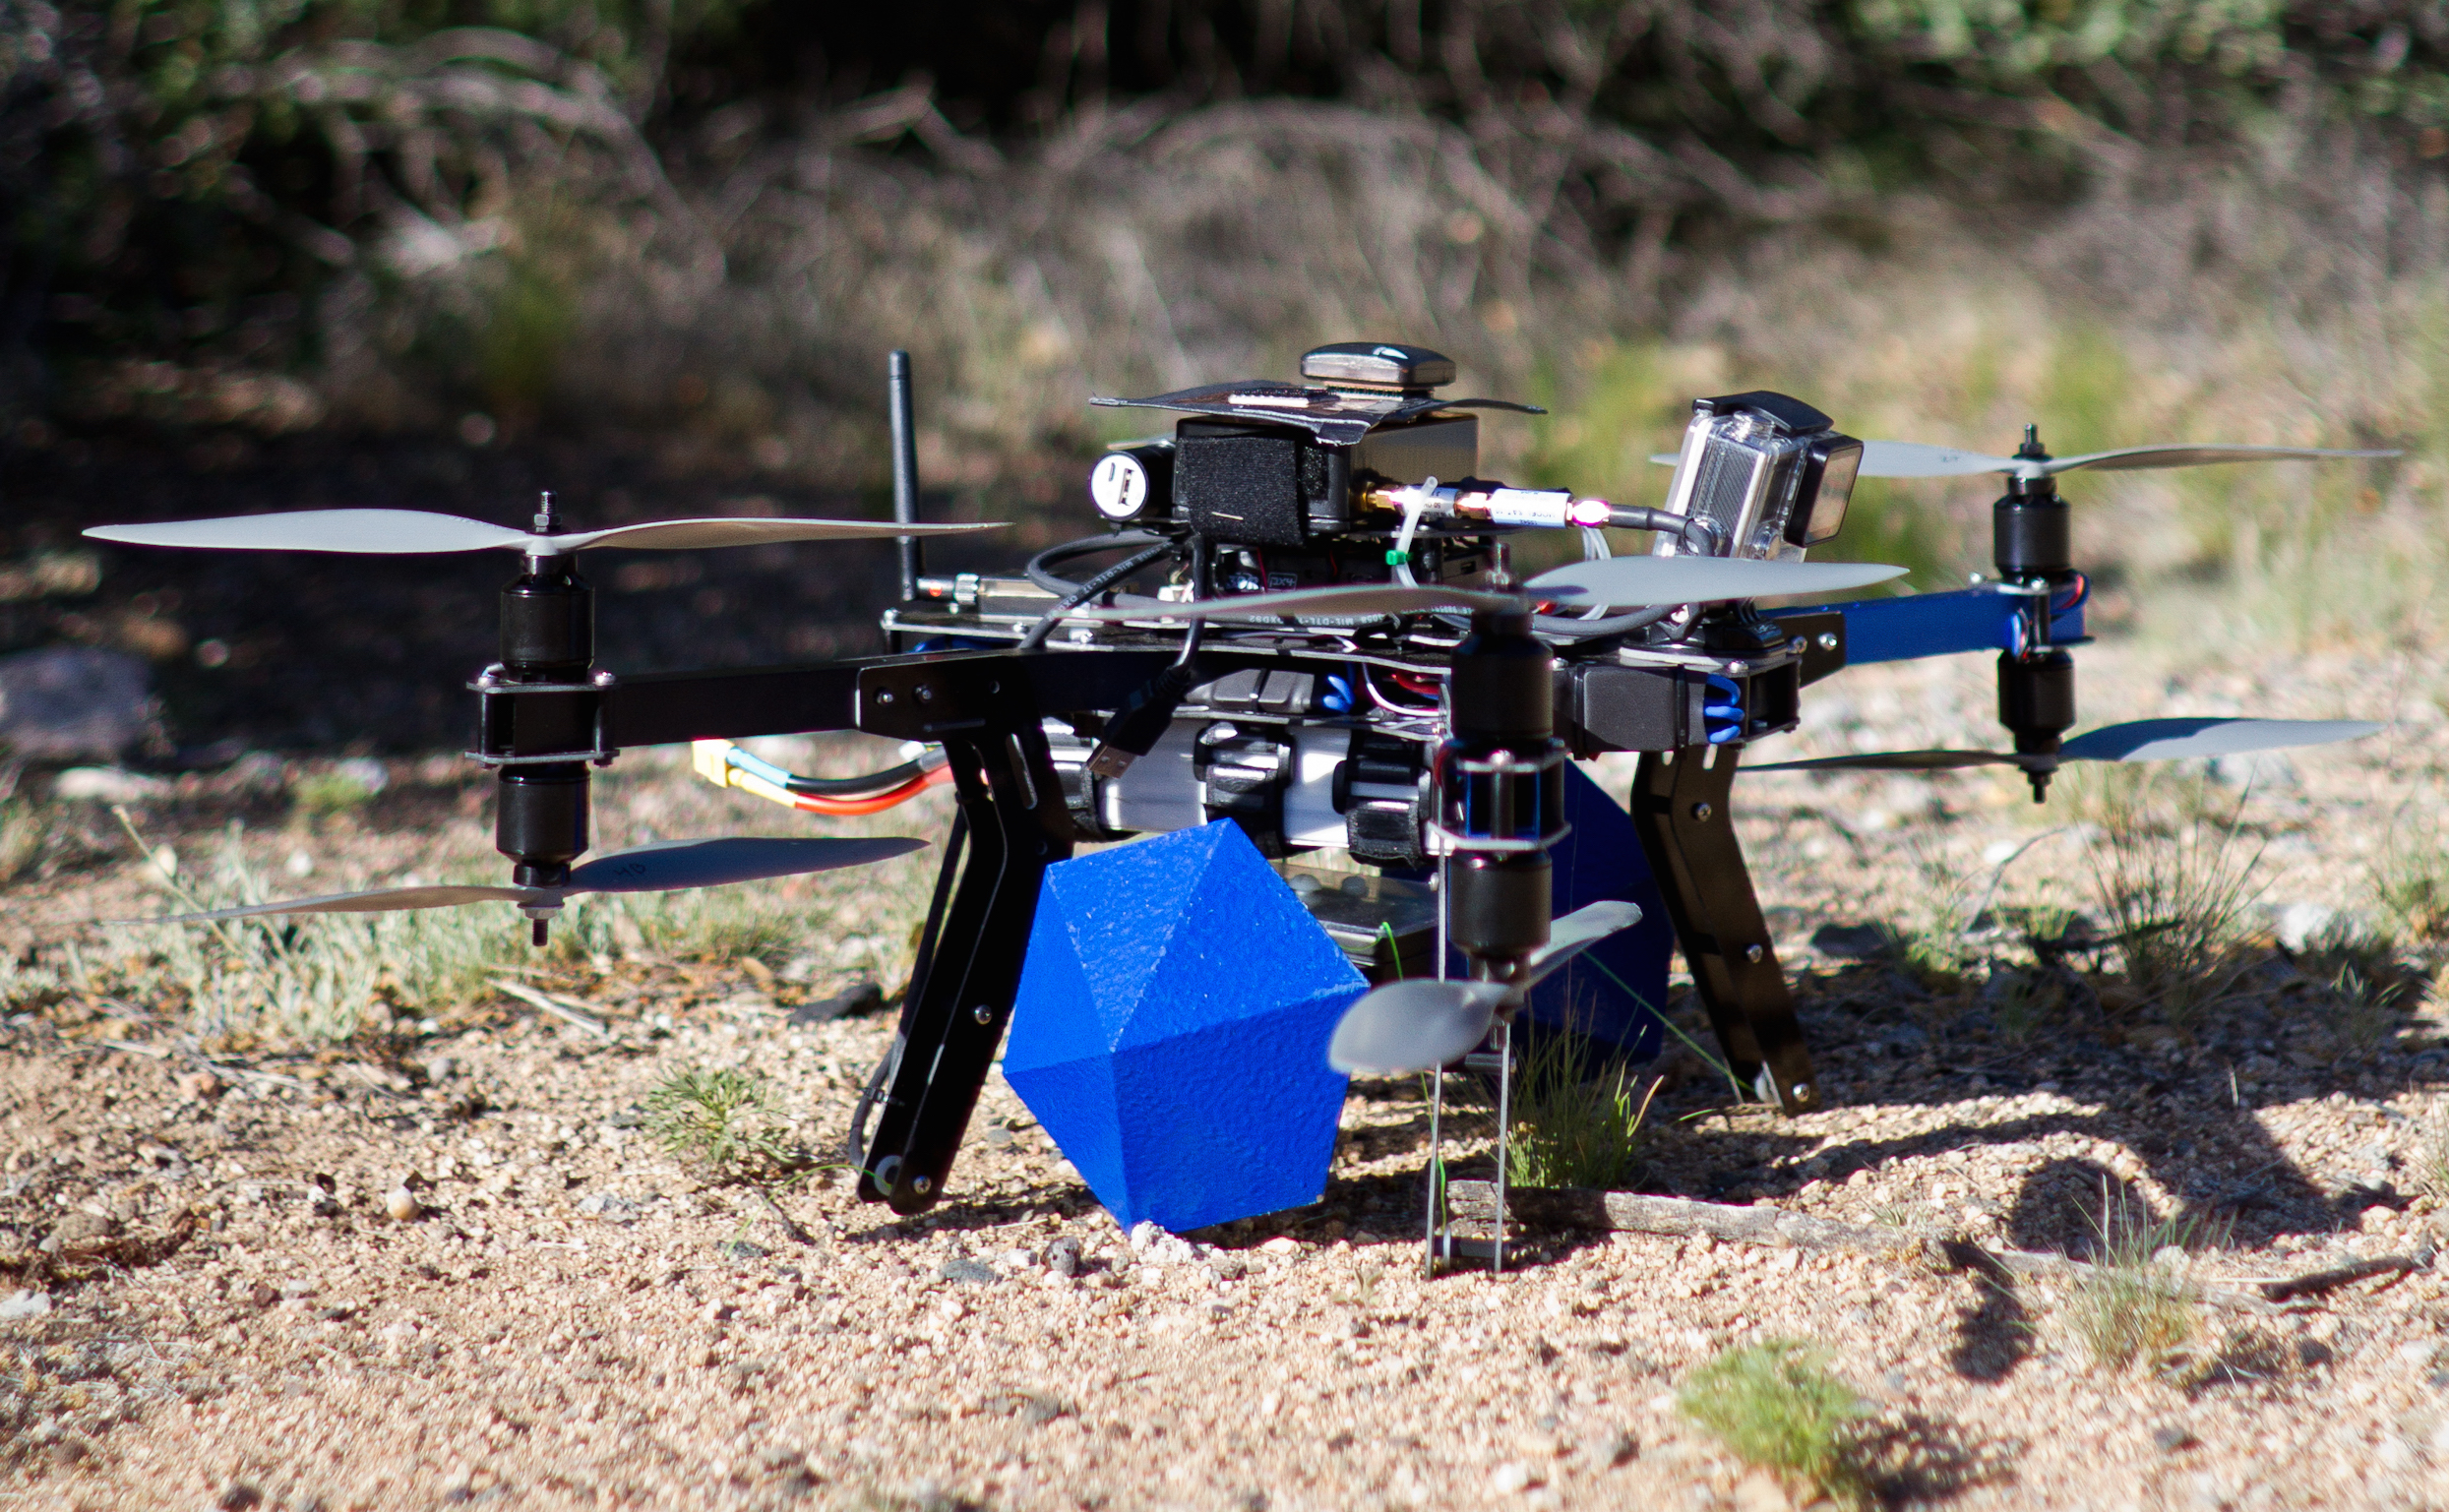
\includegraphics[scale=0.1]{images/drone2.jpg}
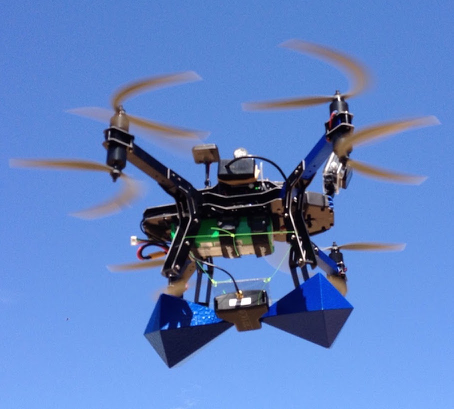
\includegraphics[scale=0.377]{images/drone.png}
\caption{3DR X8 octoquad drone prior to launch (left) and in flight (right).  The Valon synth is contained in the black project box mounted on top of the drone.  A copper plate, which acts as shielding from the electronics below, with the attached GPS magnetometer can be seen atop the project box. Beneath the drone, the BicoLOG antenna, which is blue in color, can be seen.}
\label{fig:drone}
\end{figure}

\begin{figure}[h]
\centering
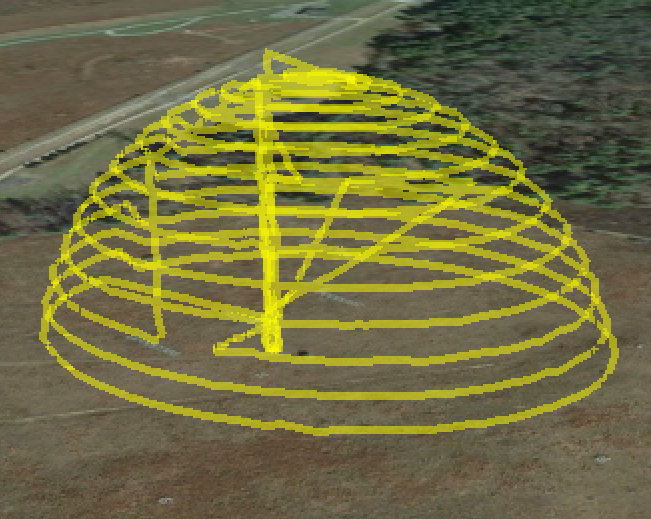
\includegraphics[scale=0.7]{images/flight_path.png}
\caption{Actual flight path of drone in Green Bank, WV.  The spiral pattern from horizon to zenith is generated from a Healpix map with parameter $N_{side}=8$.}
\label{fig:flight path}
\end{figure}

\begin{figure}[h]
\centering
\includegraphics[scale=0.4]{images/ref_ant}
\caption{Dual-polarization dipole antenna seated on a 2 m $\times$ 2 m ground screen.  Located at the NRAO Green Bank, WV site and used for ECHO testing in August, 2015.}
\label{fig:dual dipole}
\end{figure}

\end{center}

\iffalse
\begin{figure}[h]
\centering
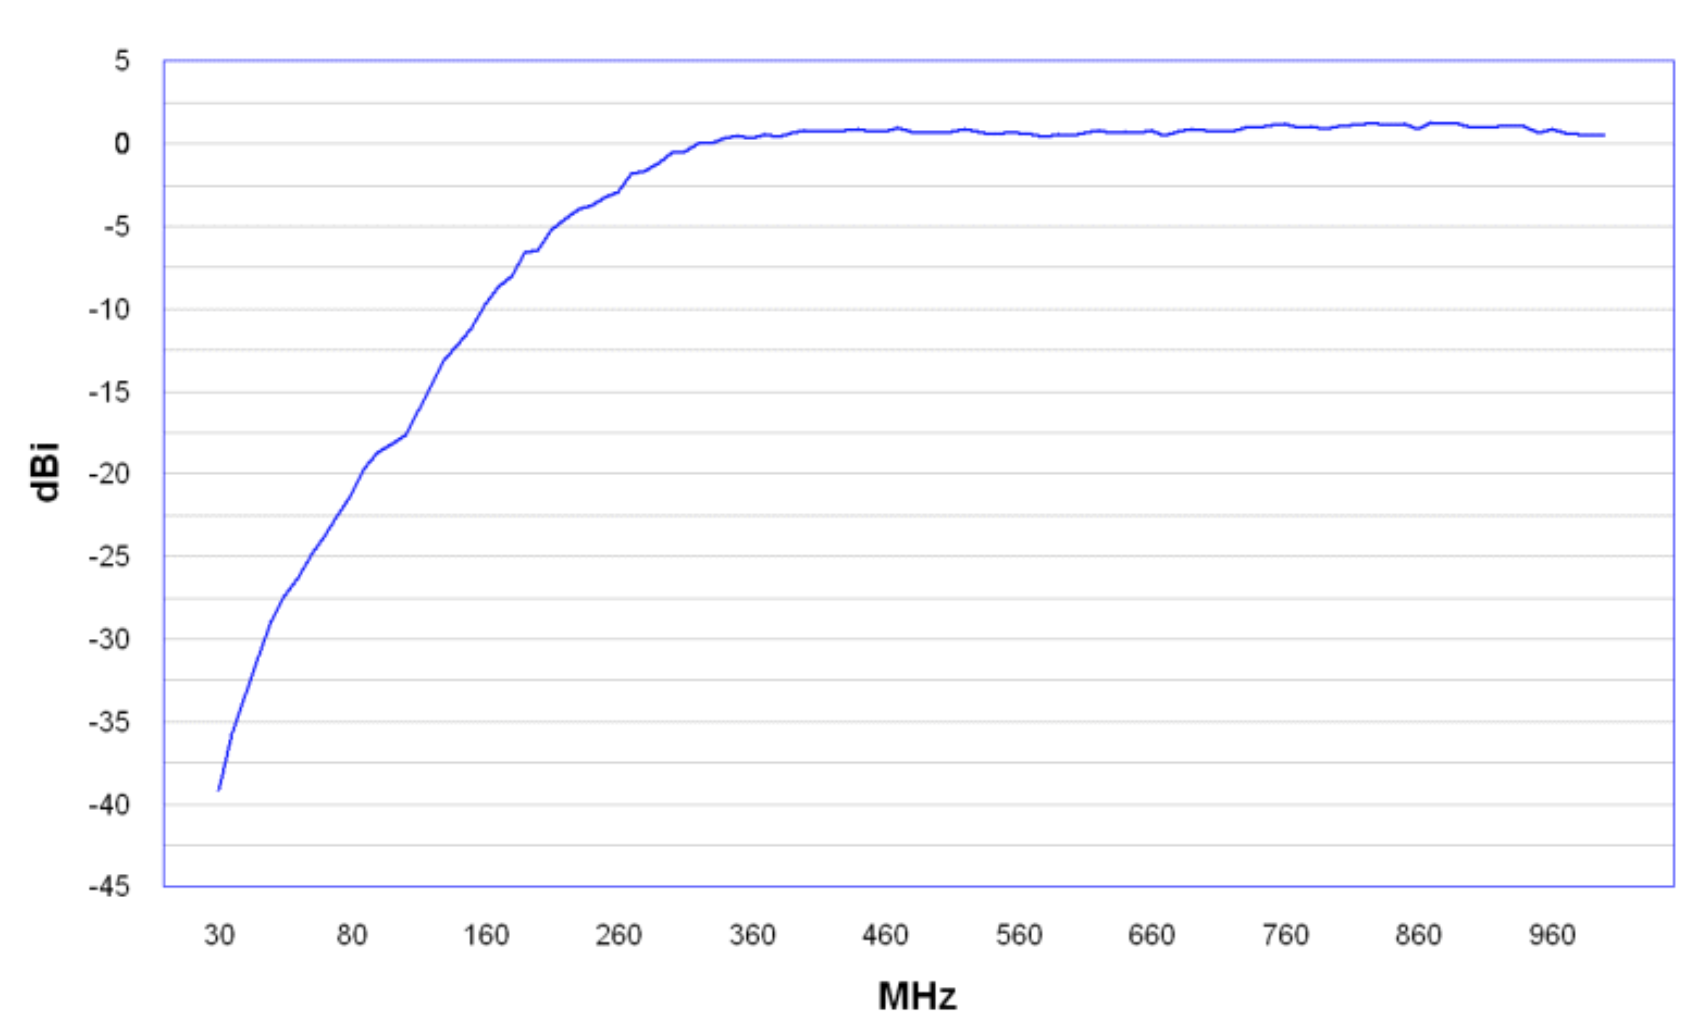
\includegraphics[scale=0.5]{images/bicolog_frequency_response.png}
\caption{Frequency response of BicoLOG 30100 biconical antenna.}
\label{BicoLOG response}
\end{figure}

\begin{figure}[h]
\centering
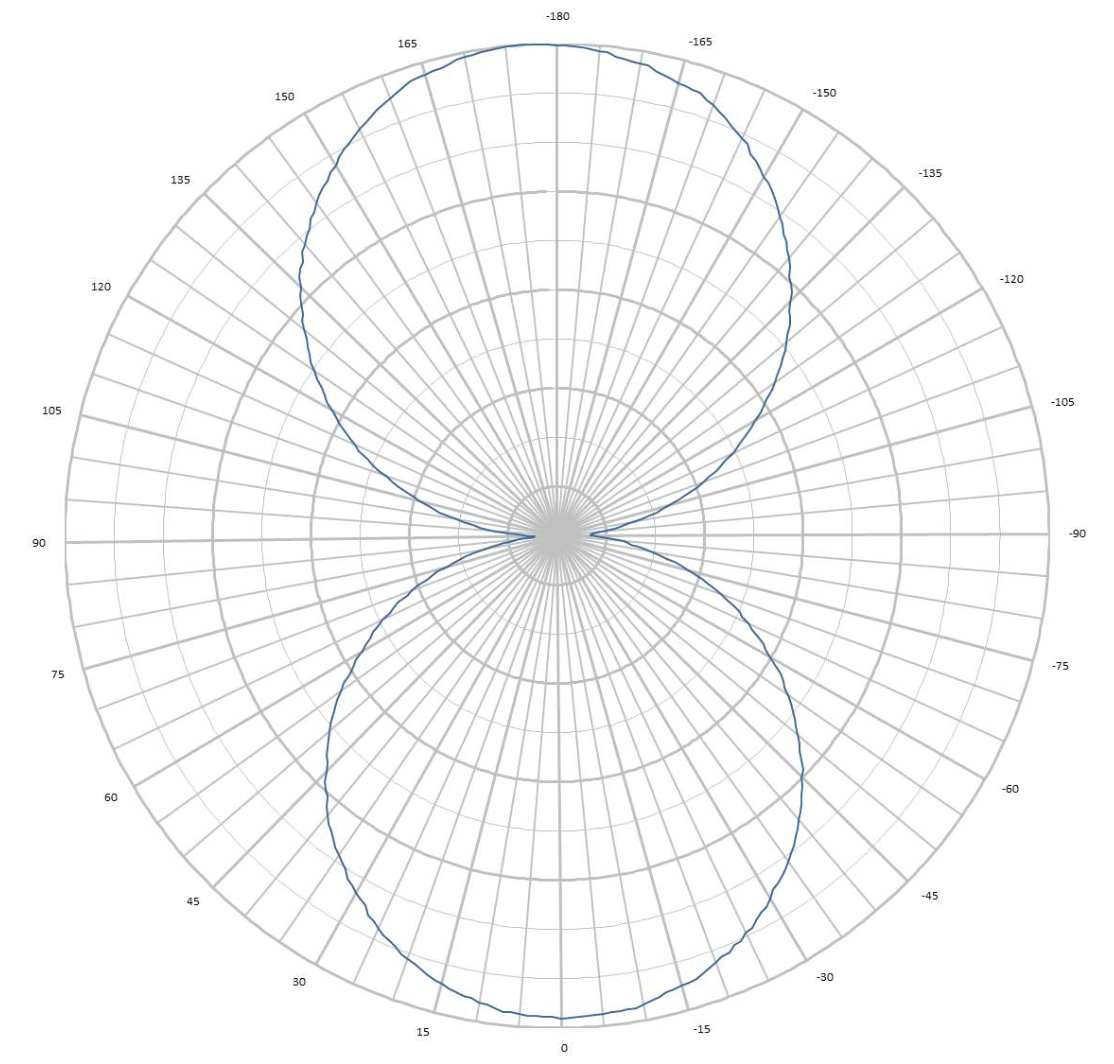
\includegraphics[scale=0.4]{images/bicolog_horizontal_cut.png}
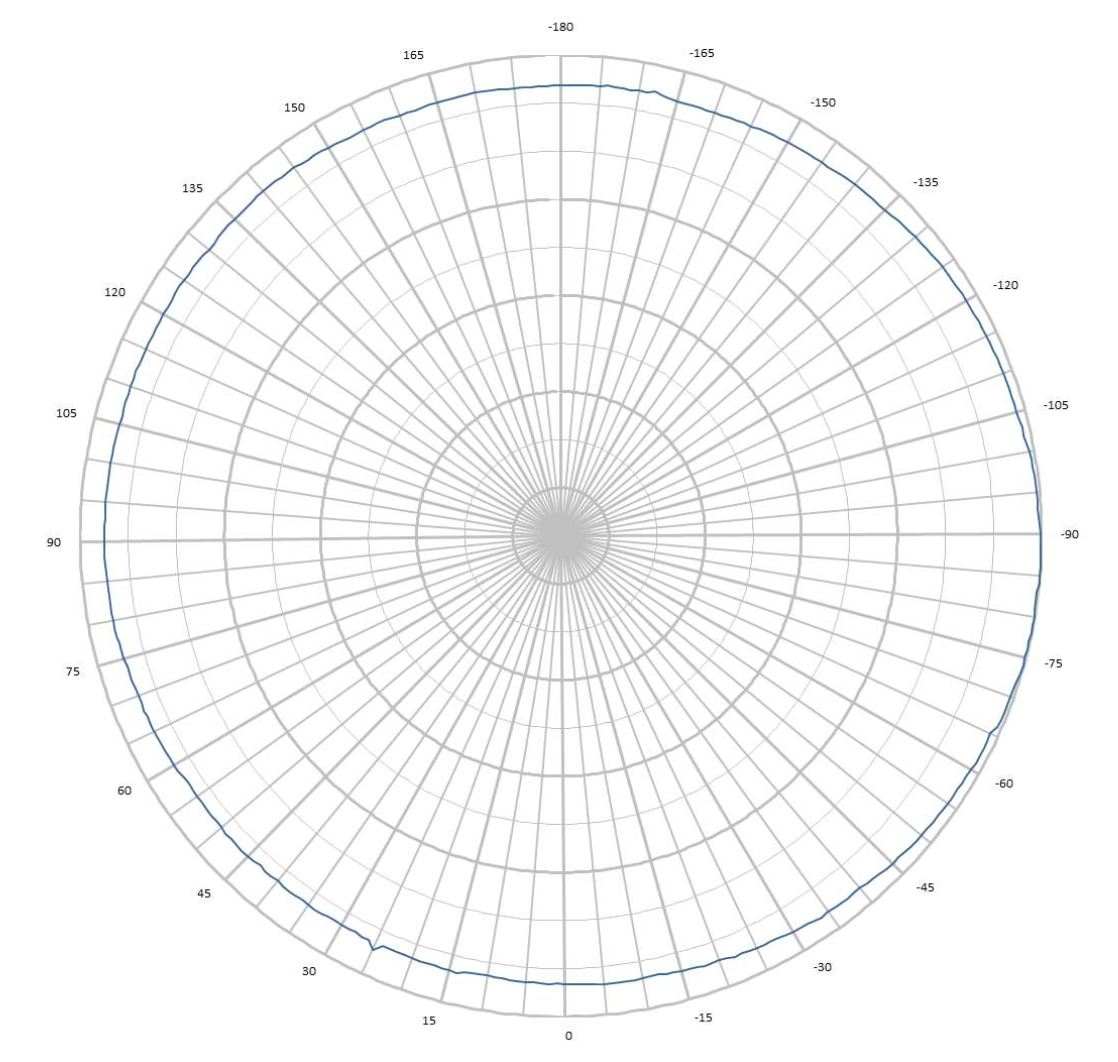
\includegraphics[scale=0.4]{images/bicolog_vertical_cut.png}
\caption{Horizontal (left) and vertical (right) cut through BicoLOG beam.}
\label{fig:BicoLOG cuts}
\end{figure}

\end{center}

\fi
\bibliography{library}
\end{document}
